\documentclass[11pt]{article}
\usepackage{header}
\def\title{HW 02}

\begin{document}
\maketitle
\fontsize{12}{15}\selectfont

\begin{center}
    Due: Saturday, 9/13, 4:00 PM \\
    Grace period until Saturday, 9/13, 6:00 PM \\
\end{center}

\section*{Sundry}
Before you start writing your final homework submission, state briefly how you worked on it.  Who else did you work with?  List names and email addresses.  (In case of homework party, you can just describe the group.)

\begin{solution}
    I worked with Lawrence Rhee (lawrencejrhee@berkeley.edu). 
    We discussed our approaches to each problem and asked each other questions.  
\end{solution}

\vspace{15pt}

\Question{Airport}

\notelinks{\href{https://www.eecs70.org/assets/pdf/notes/n3.pdf}{Note 3}}
Suppose that there are $2n+1$ airports, where $n$ is a positive integer. The distances between any two airports are all different. For each airport, exactly one airplane departs from it and is destined for the closest airport. Prove by induction that there is an airport which has no airplanes destined for it.

\begin{solution}
\begin{proof}
(Base) Let $n=1$. We have 3 airports. For any configuration of distances,
there will be a smallest distance $d$ among the finite set of distinct airport distances.
For the 2 airports being connected by this smallest distance, each will send airplanes to each other because it is the closest airport for each of them.
The single airport left that has not sent an airplane yet will end up with no planes destined to it because it can't send its airplane to itself.

(Hypothesis) Suppose for $2k+1$ airports there always exists an airport with no planes destined to it.

(Inductive step) Suppose we have $2k+3$ airports. Similar to the logic we employed in the base case,
the 2 airports connected by the smallest distance in the set of distances will send their planes to each other.
From here on out, there are 2 cases:

Case 1: as the airports send their planes to the airports, one of the airplanes
end up in one of the 2 initially matched airports. Then, an airport has 2 airplanes going into it.
Suppose every airport has at least 1 plane going into it at the end of the process.
Then we will end up with at least $2k+4$ airplanes, which is more than the number of airports we have.
This is a contradiction; therefore, in this case, there will be some airport with no planes destined to it.

Case 2: as the airports send their planes to the airports, none of the airplanes 
end up in one of the 2 initially matched airports. Then we can completely ignore the 2 matched airports.
Their distances to the other airports don't matter anymore and we can simply delete the 2 airports and their distances from the problem.
Then we end up with some $2k+1$ instance. Because in every $2k+1$ instance
an airport has no airplanes destined to it, so will $2k+3$.
\end{proof}
\end{solution} \newpage
\Question{Grid Induction}

\notelinks{\href{https://www.eecs70.org/assets/pdf/notes/n3.pdf}{Note 3}}
Pacman is walking on an infinite 2D grid.
He starts at some location $(i, j) \in \mathbb{N}^2$ in the first quadrant,
and is constrained to stay in the first quadrant (say, by walls along the $x$ and $y$ axes).

Every second he does one of the following (if possible):
\begin{enumerate}[(i)]
	\item Walk one step down, to $(i, j-1)$.
	\item Walk one step left, to $(i-1, j)$.
\end{enumerate}
For example, if he is at $(5, 0)$, his only option is to walk left to $(4, 0)$; if Pacman is instead at $(3, 2)$, he could walk either to $(2, 2)$ or $(3, 1)$.

Prove by induction that no matter how he walks, he will always reach $(0, 0)$ in finite time.

(\textit{Hint}: Try starting Pacman at a few small points like $(2, 1)$ and looking all the different paths he could take to reach $(0, 0)$.  Do you notice a pattern in the number of steps he takes? Try to use this to strengthen the inductive hypothesis.)

\begin{solution}
If Pacman starts on location $(i,j)\in\N^{2}$, he will always
land on $(0,0)$ on the $(i+j)^{th}$ second. 
Therefore, he will always reach $(0,0)$ in finite time.
\begin{proof}
(Base case) If Pacman starts on $(0,0)$ he will always land on $(0,0)$ on the $(0+0)=0^{th}$ second.

(Inductive hypothesis) If Pacman starts on any location $x,y\in\N$ where 
$x\leq i\land y\leq j\land(x,y)\neq(i,j)$,
he will always
land on $(0,0)$ on the $(x+y)^{th}$ second. 

(Inductive step) If Pacman starts on $(i,j)$, 
on the next second he will always land on either $(i,j-1)$ or $(i-1,j)$.
Because of the hypothesis, it will always take Pacman $i+j-1$ seconds to reach $(0,0)$ after the first second.
Therefore, it will always take Pacman a total of $i+j-1+1=i+j$ seconds to reach $(0,0)$.
\end{proof}
\end{solution} \newpage

\Question{Universal Preference}

\notelinks{\href{https://www.eecs70.org/assets/pdf/notes/n4.pdf}{Note 4}}
Suppose that preferences in a stable matching instance are universal: all $n$ jobs share the preferences $C_1>C_2>\cdots>C_n$ and all candidates share the preferences $J_1>J_2>\cdots>J_n$.
\begin{Parts}
    \Part What pairing do we get from running the algorithm with jobs proposing? Can you prove this happens for all $n$?
    

    \Part What pairing do we get from running the algorithm with candidates proposing?
    

    \Part What does this tell us about the number of stable pairings?
    
\end{Parts}
\begin{solution}
\begin{Parts}
\Part 
For simplicity, we will reorder the indexes in the problem statement so that the shared preferences are:
$$C_n>C_{n-1}>\dots>C_1$$
and 
$$J_n>J_{n-1}>\dots>J_1.$$
For the given restriction, the pairing
we get from running the algorithm with jobs proposing will be
$$(C_1,J_1),(C_2,J_2),\dots,(C_n,J_n)$$
over all $n$.
\begin{proof}
We prove our claim via induction.

(Base case) Let $n=1$. Then, there is only 1 matching: $(C_1,J_1)$ that can happen (and it must happen).
Therefore, the claim holds.

(Hypothesis) Let the resulting pairing for $n=k$ be 
$$(C_1,J_1),(C_2,J_2),\dots,(C_k,J_k).$$

(Inductive step) In the case of $n=k+1$, we have a 
new candidate $C_{k+1}$ and new job $J_{k+1}$ so that
for all jobs $C_{k+1}$ is more preferred than $C_k$ and
for all candidates $J_{k+1}$ is more preferred than $J_{k}$.
Then, on the first day, all the jobs will give an offer to $C_{k+1}$ 
since that is their most preferred candidate.
$C_{k+1}$ will reject all the offers except for the one from $J_{k+1}$
since that is their most preferred job. 
On any sequential day, no job will be ever offered to $C_{k+1}$
except for the one from $J_{k+1}$ because $C_{k+1}$ will be crossed from their
lists after the first day. So, after the first day, $C_{k+1}$ is 
permanently paired with $J_{k+1}$ and we can and will remove them from our instance.
We are left with the problem of $n=k$ exactly. 
The algorithm will therefore output
$$(C_1,J_1),(C_2,J_2),\dots,(C_{k+1},J_{k+1}).$$
\end{proof}
\Part By symmetry, the pairing we get from running the algorithm with candidates proposing will be the exact same result.
\Part This tells us there is only 1 stable pairing in this instance. 
This is because the job optimal (and also candidate pessimal) pairing (a) is equal to 
the candidate optimal pairing (and also job pessimal) pairing (b).
There are no "in between" matchings that are neither optimal or pessimal for any party.
Think of it as: $x\leq y$ and $x\geq y$ are both true, so $x$ must equal $y$ and there is thus only 1 possible stable matching.
\end{Parts}
\end{solution} \newpage

\Question{Pairing Up}

\notelinks{\href{https://www.eecs70.org/assets/pdf/notes/n4.pdf}{Note 4}}
Prove that for every even $n \geq 2$, there exists an instance of the stable matching problem with $n$ jobs and $n$ candidates such that the instance has at least $2^{n/2}$ distinct stable matchings.

\begin{solution}
\begin{proof}
Let's define a "2 pair" over a group of 2 candidates and 2 jobs as the following entity 
consisting of the candidates, their preferences, the jobs, and their preferences:
\begin{figure}[H]\centering
    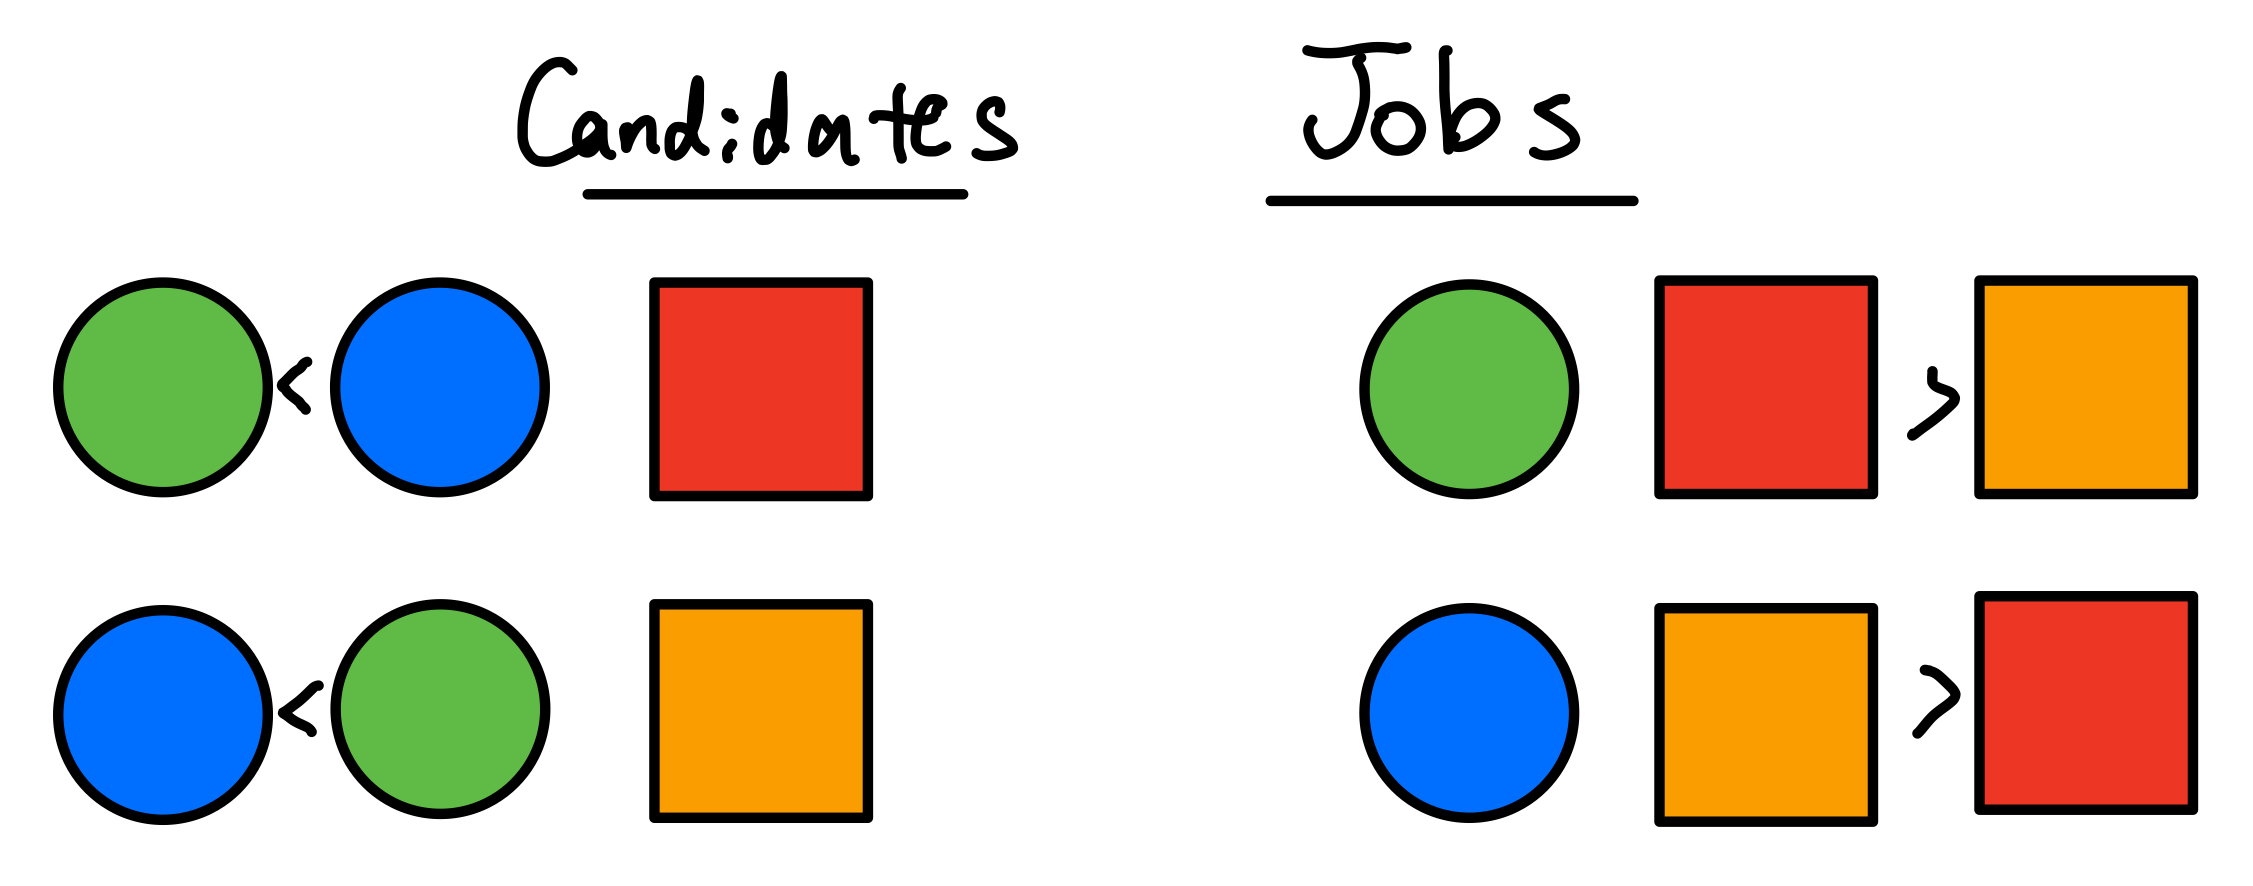
\includegraphics[width=0.4\linewidth]{assets/IMG_3276.jpg}
\end{figure}
Included in the definition of a "2 pair" is the rule that if we add a "2 pair" to an existing instance where there are already other candidates and jobs, we will make them all less preferrable then those in the group.  
\begin{figure}[H]\centering
    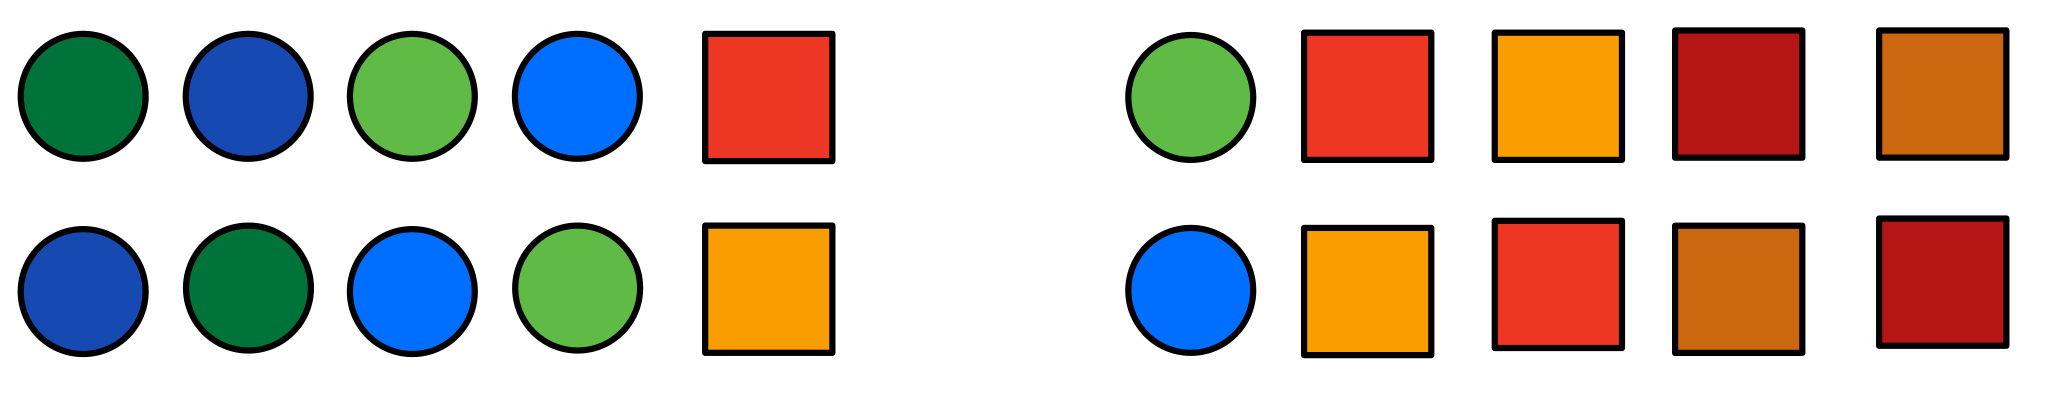
\includegraphics[width=0.6\linewidth]{assets/IMG_3278.jpg}
\end{figure}
We can see there are 2 distinct matchings within a "2 pair" regardless of how many other candidates and jobs also exist and their configurations. 
\begin{figure}[H]\centering
    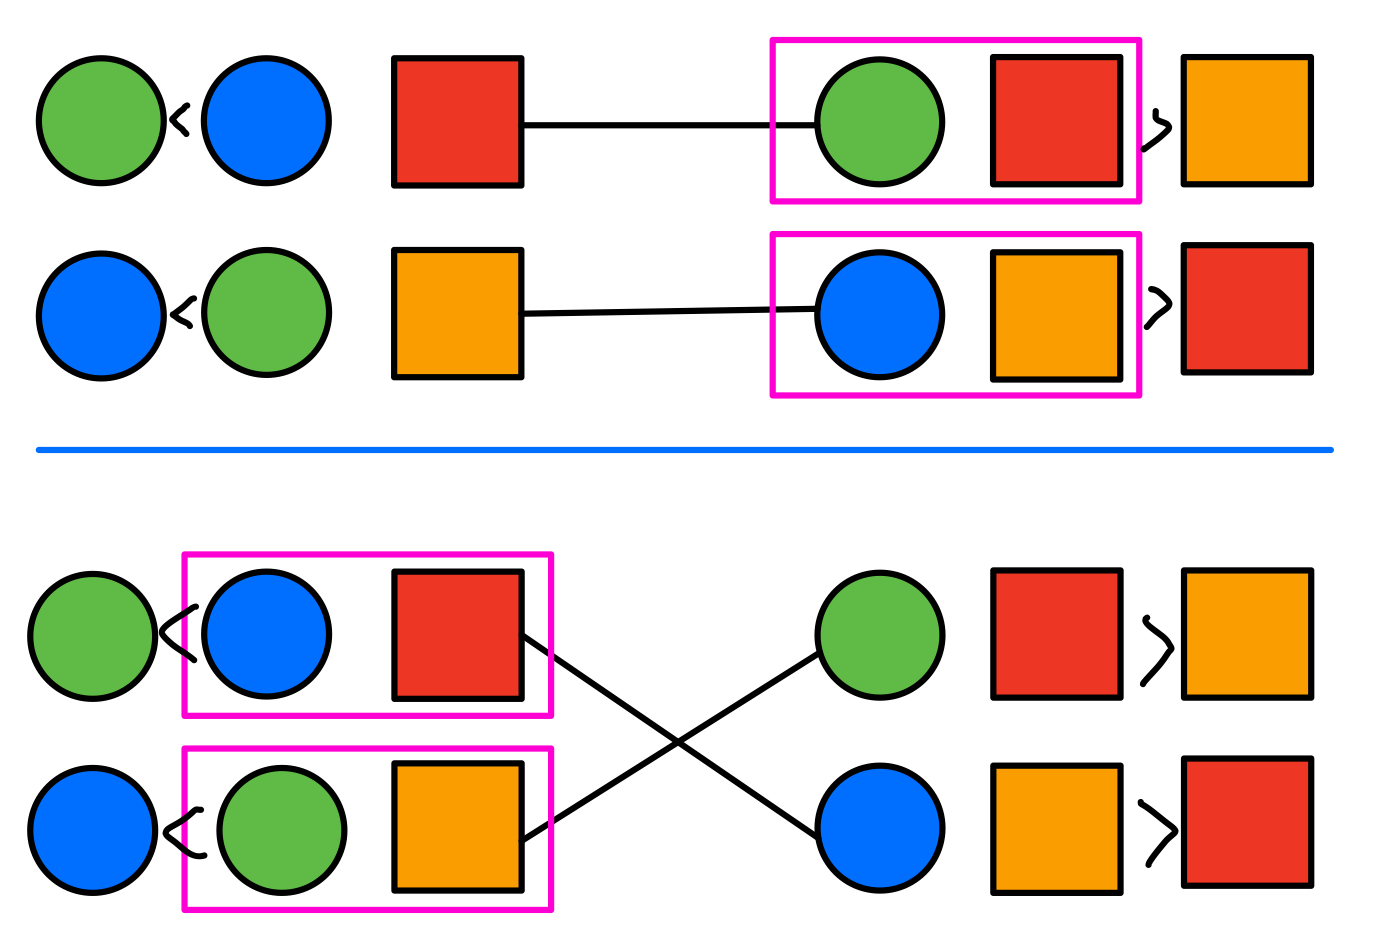
\includegraphics[width=0.4\linewidth]{assets/IMG_3275.jpg}
\end{figure}
In the top matching, the 2 jobs in the "2 pair" got their most preferred candidate so there are no rogue couples involving any job or candidate in the "2 pair".
Symmetrically, in the bottom matching, all candidates got their most preferred job, so there are no rogue couples involving any job or candidate in the "2 pair".

For positive even integer $n$, if we had an instance 
made up of only $n/2$ "2 pairs", we would have at least $2^{n/2}$ distinct stable matchings.

\end{proof}
\end{solution} \newpage

\Question{Optimal Candidates}

\notelinks{\href{https://www.eecs70.org/assets/pdf/notes/n4.pdf}{Note 4}}
In the notes, we proved that the propose-and-reject algorithm always outputs the job-optimal pairing.  However, we never explicitly showed why it is guaranteed that putting every job with its optimal candidate results in a pairing at all.  Prove by contradiction that no two jobs can have the same optimal candidate.  (Note: your proof should not rely on the fact that the propose-and-reject algorithm outputs the job-optimal pairing.)

\begin{solution}
Recall that a job's \textit{optimal candidate}
is the most preferrable candidate the job can get matched with
out of all possible stable matchings.
\begin{proof}
Suppose that 2 jobs $J$ and $J^*$ have the same optimal candidate $C$.
WLOG (without loss of generality) $C$ prefers $J$ over $J^*$ (can't have equal preference for 2 different jobs). 
Then, there exists some stable matching that contains the pair $(J,C)$ (when $J$ gets its optimal candidate)
and there also exists some stable matching that contains the pair $(J^*,C)$ (when $J^*$ gets its optimal candidate).
Then, in the stable matching containing $(J^*,C)$,
$J$ is paired with a candidate it prefers less than $C$, ($C$ is the best it can get, so in any stable matching $J$ is not with $C$ it is with someone less preferred than $C$).
$C$ also prefers $J$ over $J^*$ as established earlier.
Then, we have a rogue couple. Thus, the matching is not stable and 
we have a contradiction because we've already established this to be a stable matching.
\end{proof}
\end{solution}

\end{document}

%UNNECESSARY AIRPLANE YAP%
%0.
% The problem statement is analogous to an undirected graph with 
% airport $i$ being denoted as node $i$ and every node is connected to every other node.
% Each edge has a unique length characteristic (distance between the 2 connected airports).
%1.
% We define $P(n)$ as the proposition that 
% there is an airport which has no airplanes destined for it for any configuration of the distances (distinct) 
% for $2n+1$ airports, where $n$ is a positive integer.
% We will prove via induction that $P(n)$ is true for all positive integers $n$.
%2.
% \begin{tikzpicture}[->,>=stealth',shorten >=1pt,auto,node distance=3cm,
%     thick,main node/.style={circle,draw,font=\sffamily\Large\bfseries}]

% \node[main node] (1) {1};
% \node[main node] (2) [below left of=1] {2};
% \node[main node] (3) [below right of=1] {3};

% \path[every node/.style={font=\sffamily\small}]
% (1) 
% edge[bend right] node {0.3} (2)
% edge[bend right] node {0.3} (3)
% (2) 
% edge[bend right] node {0.3} (1)
% edge[bend right] node {0.4} (3)
% (3) 
% edge[bend right] node {0.8} (1)
% edge[bend right] node {0.3} (2);
% \end{tikzpicture}

%UNNECESSARY MATCHING YAP%
%  we had only 1 "2 pair", we would have 2 distinct stable matchings.
% This satisfies $2^{2/2}=2$.
% Let's now suppose we have an instance for $n=k$ (positive even integer $k$) where the instance has at least $2^{k/2}$ distinct stable matchings
% and is composed of only "2 pair"s.
% By the definition and properties of a "2 pair", if we were to add another "2 pair",
% We would have at least twice the amount of distinct stable matchings. 
% The new "2 pair" would not remove 
% Now, assume we have an instance for $n=2k$ for positive integer $k$ where there are at least $2^{k/2}$ distinct matchings.
% Let's add a new "2 pair", 2 new jobs, where we make them both less preferrable (in any order) than the most preffered job for each candidate.
% Similarly, let's add 2 new candidates, where we make them both less preferrable (in any order) than the most preffered candidate for each job.
% In this manner, we will not remove any of the previous distinct matchings we've already created.
% Each "2 pair" will still have at least 2 distinct matchings independent of the other "2 pair"s.
% Each previous candidate 
% When we add 2 new candidates, we will make them both less preferrable than the 2 current candidates for the $n=2$ scenario.
% As long as when we add new candidates and jobs we do not "mess with" the old
% candidates and jobs preferences (i.e.)
% The first 2 jobs and 2 candidates from $n=2$ will always have 2 options:
% the candidates get their top choices 
% If we add 2 more jobs and 2 more candidates to our instance,
% we can configure them 